% Options for packages loaded elsewhere
\PassOptionsToPackage{unicode}{hyperref}
\PassOptionsToPackage{hyphens}{url}
\PassOptionsToPackage{dvipsnames,svgnames,x11names}{xcolor}
%
\documentclass[
  letterpaper,
  DIV=11,
  numbers=noendperiod]{scrartcl}

\usepackage{amsmath,amssymb}
\usepackage{iftex}
\ifPDFTeX
  \usepackage[T1]{fontenc}
  \usepackage[utf8]{inputenc}
  \usepackage{textcomp} % provide euro and other symbols
\else % if luatex or xetex
  \usepackage{unicode-math}
  \defaultfontfeatures{Scale=MatchLowercase}
  \defaultfontfeatures[\rmfamily]{Ligatures=TeX,Scale=1}
\fi
\usepackage{lmodern}
\ifPDFTeX\else  
    % xetex/luatex font selection
\fi
% Use upquote if available, for straight quotes in verbatim environments
\IfFileExists{upquote.sty}{\usepackage{upquote}}{}
\IfFileExists{microtype.sty}{% use microtype if available
  \usepackage[]{microtype}
  \UseMicrotypeSet[protrusion]{basicmath} % disable protrusion for tt fonts
}{}
\makeatletter
\@ifundefined{KOMAClassName}{% if non-KOMA class
  \IfFileExists{parskip.sty}{%
    \usepackage{parskip}
  }{% else
    \setlength{\parindent}{0pt}
    \setlength{\parskip}{6pt plus 2pt minus 1pt}}
}{% if KOMA class
  \KOMAoptions{parskip=half}}
\makeatother
\usepackage{xcolor}
\setlength{\emergencystretch}{3em} % prevent overfull lines
\setcounter{secnumdepth}{-\maxdimen} % remove section numbering
% Make \paragraph and \subparagraph free-standing
\ifx\paragraph\undefined\else
  \let\oldparagraph\paragraph
  \renewcommand{\paragraph}[1]{\oldparagraph{#1}\mbox{}}
\fi
\ifx\subparagraph\undefined\else
  \let\oldsubparagraph\subparagraph
  \renewcommand{\subparagraph}[1]{\oldsubparagraph{#1}\mbox{}}
\fi

\usepackage{color}
\usepackage{fancyvrb}
\newcommand{\VerbBar}{|}
\newcommand{\VERB}{\Verb[commandchars=\\\{\}]}
\DefineVerbatimEnvironment{Highlighting}{Verbatim}{commandchars=\\\{\}}
% Add ',fontsize=\small' for more characters per line
\usepackage{framed}
\definecolor{shadecolor}{RGB}{241,243,245}
\newenvironment{Shaded}{\begin{snugshade}}{\end{snugshade}}
\newcommand{\AlertTok}[1]{\textcolor[rgb]{0.68,0.00,0.00}{#1}}
\newcommand{\AnnotationTok}[1]{\textcolor[rgb]{0.37,0.37,0.37}{#1}}
\newcommand{\AttributeTok}[1]{\textcolor[rgb]{0.40,0.45,0.13}{#1}}
\newcommand{\BaseNTok}[1]{\textcolor[rgb]{0.68,0.00,0.00}{#1}}
\newcommand{\BuiltInTok}[1]{\textcolor[rgb]{0.00,0.23,0.31}{#1}}
\newcommand{\CharTok}[1]{\textcolor[rgb]{0.13,0.47,0.30}{#1}}
\newcommand{\CommentTok}[1]{\textcolor[rgb]{0.37,0.37,0.37}{#1}}
\newcommand{\CommentVarTok}[1]{\textcolor[rgb]{0.37,0.37,0.37}{\textit{#1}}}
\newcommand{\ConstantTok}[1]{\textcolor[rgb]{0.56,0.35,0.01}{#1}}
\newcommand{\ControlFlowTok}[1]{\textcolor[rgb]{0.00,0.23,0.31}{#1}}
\newcommand{\DataTypeTok}[1]{\textcolor[rgb]{0.68,0.00,0.00}{#1}}
\newcommand{\DecValTok}[1]{\textcolor[rgb]{0.68,0.00,0.00}{#1}}
\newcommand{\DocumentationTok}[1]{\textcolor[rgb]{0.37,0.37,0.37}{\textit{#1}}}
\newcommand{\ErrorTok}[1]{\textcolor[rgb]{0.68,0.00,0.00}{#1}}
\newcommand{\ExtensionTok}[1]{\textcolor[rgb]{0.00,0.23,0.31}{#1}}
\newcommand{\FloatTok}[1]{\textcolor[rgb]{0.68,0.00,0.00}{#1}}
\newcommand{\FunctionTok}[1]{\textcolor[rgb]{0.28,0.35,0.67}{#1}}
\newcommand{\ImportTok}[1]{\textcolor[rgb]{0.00,0.46,0.62}{#1}}
\newcommand{\InformationTok}[1]{\textcolor[rgb]{0.37,0.37,0.37}{#1}}
\newcommand{\KeywordTok}[1]{\textcolor[rgb]{0.00,0.23,0.31}{#1}}
\newcommand{\NormalTok}[1]{\textcolor[rgb]{0.00,0.23,0.31}{#1}}
\newcommand{\OperatorTok}[1]{\textcolor[rgb]{0.37,0.37,0.37}{#1}}
\newcommand{\OtherTok}[1]{\textcolor[rgb]{0.00,0.23,0.31}{#1}}
\newcommand{\PreprocessorTok}[1]{\textcolor[rgb]{0.68,0.00,0.00}{#1}}
\newcommand{\RegionMarkerTok}[1]{\textcolor[rgb]{0.00,0.23,0.31}{#1}}
\newcommand{\SpecialCharTok}[1]{\textcolor[rgb]{0.37,0.37,0.37}{#1}}
\newcommand{\SpecialStringTok}[1]{\textcolor[rgb]{0.13,0.47,0.30}{#1}}
\newcommand{\StringTok}[1]{\textcolor[rgb]{0.13,0.47,0.30}{#1}}
\newcommand{\VariableTok}[1]{\textcolor[rgb]{0.07,0.07,0.07}{#1}}
\newcommand{\VerbatimStringTok}[1]{\textcolor[rgb]{0.13,0.47,0.30}{#1}}
\newcommand{\WarningTok}[1]{\textcolor[rgb]{0.37,0.37,0.37}{\textit{#1}}}

\providecommand{\tightlist}{%
  \setlength{\itemsep}{0pt}\setlength{\parskip}{0pt}}\usepackage{longtable,booktabs,array}
\usepackage{calc} % for calculating minipage widths
% Correct order of tables after \paragraph or \subparagraph
\usepackage{etoolbox}
\makeatletter
\patchcmd\longtable{\par}{\if@noskipsec\mbox{}\fi\par}{}{}
\makeatother
% Allow footnotes in longtable head/foot
\IfFileExists{footnotehyper.sty}{\usepackage{footnotehyper}}{\usepackage{footnote}}
\makesavenoteenv{longtable}
\usepackage{graphicx}
\makeatletter
\def\maxwidth{\ifdim\Gin@nat@width>\linewidth\linewidth\else\Gin@nat@width\fi}
\def\maxheight{\ifdim\Gin@nat@height>\textheight\textheight\else\Gin@nat@height\fi}
\makeatother
% Scale images if necessary, so that they will not overflow the page
% margins by default, and it is still possible to overwrite the defaults
% using explicit options in \includegraphics[width, height, ...]{}
\setkeys{Gin}{width=\maxwidth,height=\maxheight,keepaspectratio}
% Set default figure placement to htbp
\makeatletter
\def\fps@figure{htbp}
\makeatother

\KOMAoption{captions}{tableheading}
\makeatletter
\makeatother
\makeatletter
\makeatother
\makeatletter
\@ifpackageloaded{caption}{}{\usepackage{caption}}
\AtBeginDocument{%
\ifdefined\contentsname
  \renewcommand*\contentsname{Table of contents}
\else
  \newcommand\contentsname{Table of contents}
\fi
\ifdefined\listfigurename
  \renewcommand*\listfigurename{List of Figures}
\else
  \newcommand\listfigurename{List of Figures}
\fi
\ifdefined\listtablename
  \renewcommand*\listtablename{List of Tables}
\else
  \newcommand\listtablename{List of Tables}
\fi
\ifdefined\figurename
  \renewcommand*\figurename{Figure}
\else
  \newcommand\figurename{Figure}
\fi
\ifdefined\tablename
  \renewcommand*\tablename{Table}
\else
  \newcommand\tablename{Table}
\fi
}
\@ifpackageloaded{float}{}{\usepackage{float}}
\floatstyle{ruled}
\@ifundefined{c@chapter}{\newfloat{codelisting}{h}{lop}}{\newfloat{codelisting}{h}{lop}[chapter]}
\floatname{codelisting}{Listing}
\newcommand*\listoflistings{\listof{codelisting}{List of Listings}}
\makeatother
\makeatletter
\@ifpackageloaded{caption}{}{\usepackage{caption}}
\@ifpackageloaded{subcaption}{}{\usepackage{subcaption}}
\makeatother
\makeatletter
\@ifpackageloaded{tcolorbox}{}{\usepackage[skins,breakable]{tcolorbox}}
\makeatother
\makeatletter
\@ifundefined{shadecolor}{\definecolor{shadecolor}{rgb}{.97, .97, .97}}
\makeatother
\makeatletter
\makeatother
\makeatletter
\makeatother
\ifLuaTeX
  \usepackage{selnolig}  % disable illegal ligatures
\fi
\IfFileExists{bookmark.sty}{\usepackage{bookmark}}{\usepackage{hyperref}}
\IfFileExists{xurl.sty}{\usepackage{xurl}}{} % add URL line breaks if available
\urlstyle{same} % disable monospaced font for URLs
\hypersetup{
  pdftitle={Prospective UK undergraduate attitudes towards Theology and Religious Studies},
  pdfauthor={Jeremy H. Kidwell},
  colorlinks=true,
  linkcolor={blue},
  filecolor={Maroon},
  citecolor={Blue},
  urlcolor={Blue},
  pdfcreator={LaTeX via pandoc}}

\title{Prospective UK undergraduate attitudes towards Theology and
Religious Studies}
\author{Jeremy H. Kidwell}
\date{}

\begin{document}
\maketitle
\ifdefined\Shaded\renewenvironment{Shaded}{\begin{tcolorbox}[sharp corners, breakable, frame hidden, enhanced, boxrule=0pt, interior hidden, borderline west={3pt}{0pt}{shadecolor}]}{\end{tcolorbox}}\fi

\begin{Shaded}
\begin{Highlighting}[]
\FunctionTok{library}\NormalTok{(ggplot2)}
\FunctionTok{library}\NormalTok{(usethis)}
\FunctionTok{library}\NormalTok{(devtools)}
\FunctionTok{library}\NormalTok{(likert)}
\end{Highlighting}
\end{Shaded}

\begin{verbatim}
Loading required package: xtable
\end{verbatim}

\begin{Shaded}
\begin{Highlighting}[]
\FunctionTok{library}\NormalTok{(RColorBrewer)}
\FunctionTok{library}\NormalTok{(}\StringTok{"readxl"}\NormalTok{)}
\FunctionTok{library}\NormalTok{(haven)}
\FunctionTok{library}\NormalTok{(scales)}
\FunctionTok{library}\NormalTok{(tidyverse)}
\end{Highlighting}
\end{Shaded}

\begin{verbatim}
-- Attaching core tidyverse packages ------------------------ tidyverse 2.0.0 --
v dplyr     1.1.4     v readr     2.1.5
v forcats   1.0.0     v stringr   1.5.1
v lubridate 1.9.3     v tibble    3.2.1
v purrr     1.0.2     v tidyr     1.3.1
\end{verbatim}

\begin{verbatim}
-- Conflicts ------------------------------------------ tidyverse_conflicts() --
x readr::col_factor() masks scales::col_factor()
x purrr::discard()    masks scales::discard()
x dplyr::filter()     masks stats::filter()
x dplyr::lag()        masks stats::lag()
x dplyr::recode()     masks likert::recode()
i Use the conflicted package (<http://conflicted.r-lib.org/>) to force all conflicts to become errors
\end{verbatim}

\begin{Shaded}
\begin{Highlighting}[]
\CommentTok{\# Define colour palettes for plots below}
\NormalTok{coul3 }\OtherTok{\textless{}{-}} \FunctionTok{brewer.pal}\NormalTok{(}\DecValTok{3}\NormalTok{, }\StringTok{"RdYlBu"}\NormalTok{) }\CommentTok{\# Using RdYlBu range to generate 3 colour palette: https://colorbrewer2.org/\#type=diverging\&scheme=RdYlBu\&n=5}

\NormalTok{subject\_data }\OtherTok{\textless{}{-}} \FunctionTok{read.csv}\NormalTok{(}\StringTok{"./data/Subject data.csv"}\NormalTok{)}
\NormalTok{admissions\_data }\OtherTok{\textless{}{-}} \FunctionTok{read\_excel}\NormalTok{(}\StringTok{"./data/TSR\_data\_numbers.xlsx"}\NormalTok{, }\AttributeTok{sheet =} \StringTok{"Raw data {-} completes"}\NormalTok{)}

\CommentTok{\# Set up local workspace, as needed:}

\ControlFlowTok{if}\NormalTok{ (}\FunctionTok{dir.exists}\NormalTok{(}\StringTok{"data"}\NormalTok{) }\SpecialCharTok{==} \ConstantTok{FALSE}\NormalTok{) \{}
  \FunctionTok{dir.create}\NormalTok{(}\StringTok{"data"}\NormalTok{) }
\NormalTok{\}}

\CommentTok{\# These paths are excluded from github as it is best practice for end{-}user to generate their own}

\ControlFlowTok{if}\NormalTok{ (}\FunctionTok{dir.exists}\NormalTok{(}\StringTok{"figures"}\NormalTok{) }\SpecialCharTok{==} \ConstantTok{FALSE}\NormalTok{) \{}
  \FunctionTok{dir.create}\NormalTok{(}\StringTok{"figures"}\NormalTok{) }
\NormalTok{\}}
\ControlFlowTok{if}\NormalTok{ (}\FunctionTok{dir.exists}\NormalTok{(}\StringTok{"derivedData"}\NormalTok{) }\SpecialCharTok{==} \ConstantTok{FALSE}\NormalTok{) \{}
  \FunctionTok{dir.create}\NormalTok{(}\StringTok{"derivedData"}\NormalTok{)}
\NormalTok{\}}

\CommentTok{\# Refactor data}
\NormalTok{admissions\_data}\SpecialCharTok{$}\NormalTok{Q2 }\OtherTok{\textless{}{-}} \FunctionTok{labelled}\NormalTok{(admissions\_data}\SpecialCharTok{$}\NormalTok{Q2, }\FunctionTok{c}\NormalTok{(}\StringTok{"15 or under"} \OtherTok{=} \DecValTok{1}\NormalTok{, }\StringTok{"16"} \OtherTok{=} \DecValTok{2}\NormalTok{, }\StringTok{"17"} \OtherTok{=} \DecValTok{3}\NormalTok{, }\StringTok{"18"} \OtherTok{=} \DecValTok{4}\NormalTok{, }\StringTok{"19"} \OtherTok{=} \DecValTok{5}\NormalTok{, }\StringTok{"20"} \OtherTok{=} \DecValTok{6}\NormalTok{, }\StringTok{"21 or over"} \OtherTok{=} \DecValTok{7}\NormalTok{, }\StringTok{"Prefer not to say"} \OtherTok{=} \DecValTok{8}\NormalTok{), }\AttributeTok{label =} \StringTok{"How old are you?"}\NormalTok{)}

\NormalTok{admissions\_data}\SpecialCharTok{$}\NormalTok{Q3 }\OtherTok{\textless{}{-}} \FunctionTok{labelled}\NormalTok{(admissions\_data}\SpecialCharTok{$}\NormalTok{Q3, }\FunctionTok{c}\NormalTok{(}\StringTok{"Year 11/S4/Year 12(NI)"} \OtherTok{=} \DecValTok{1}\NormalTok{, }\StringTok{"Year 12/S5/Year 13(NI)"} \OtherTok{=} \DecValTok{2}\NormalTok{, }\StringTok{"Year 13/S6/Year 14(NI)"} \OtherTok{=} \DecValTok{3}\NormalTok{, }\StringTok{"I am currently on a gap year"} \OtherTok{=} \DecValTok{4}\NormalTok{, }\StringTok{"I am currently on an undergraduate/HE college course"} \OtherTok{=} \DecValTok{5}\NormalTok{, }\StringTok{"I am in full{-}time employment"} \OtherTok{=} \DecValTok{6}\NormalTok{, }\StringTok{"I am unemployed"} \OtherTok{=} \DecValTok{7}\NormalTok{, }\StringTok{"Other"} \OtherTok{=} \DecValTok{8}\NormalTok{, }\StringTok{"Prefer not to say"} \OtherTok{=} \DecValTok{9}\NormalTok{), }\AttributeTok{label =} \StringTok{"Which of the following best describes your MOST RECENT year of study?"}\NormalTok{)}

\NormalTok{admissions\_data}\SpecialCharTok{$}\NormalTok{Q4 }\OtherTok{\textless{}{-}} \FunctionTok{labelled}\NormalTok{(admissions\_data}\SpecialCharTok{$}\NormalTok{Q4, }\FunctionTok{c}\NormalTok{(}\StringTok{"Yes, definitely"} \OtherTok{=} \DecValTok{1}\NormalTok{, }\StringTok{"Yes, probably"} \OtherTok{=} \DecValTok{2}\NormalTok{, }\StringTok{"I haven’t ruled it out"} \OtherTok{=} \DecValTok{3}\NormalTok{), }\AttributeTok{label =} \StringTok{"Are you considering or planning to go to university in the future?"}\NormalTok{)}

\NormalTok{common\_labels }\OtherTok{\textless{}{-}} \FunctionTok{c}\NormalTok{(}
  \StringTok{"Strongly agree"} \OtherTok{=} \DecValTok{1}\NormalTok{,}
  \StringTok{"Agree"} \OtherTok{=} \DecValTok{2}\NormalTok{,}
  \StringTok{"Neither/Nor"} \OtherTok{=} \DecValTok{3}\NormalTok{,}
  \StringTok{"Disagree"} \OtherTok{=} \DecValTok{4}\NormalTok{,}
  \StringTok{"Strongly disagree"} \OtherTok{=} \DecValTok{5}\NormalTok{,}
  \StringTok{"Prefer not to say"} \OtherTok{=} \DecValTok{0}
\NormalTok{)}

\NormalTok{admissions\_data }\OtherTok{\textless{}{-}}\NormalTok{ admissions\_data }\SpecialCharTok{\%\textgreater{}\%}
  \FunctionTok{mutate\_at}\NormalTok{(}\FunctionTok{vars}\NormalTok{(}\FunctionTok{starts\_with}\NormalTok{(}\StringTok{"Q5\_"}\NormalTok{)), }\SpecialCharTok{\textasciitilde{}} \FunctionTok{labelled}\NormalTok{(., common\_labels, }\AttributeTok{label =} \StringTok{"I have a good understanding of what this subject involves"}\NormalTok{))}

\NormalTok{admissions\_data }\OtherTok{\textless{}{-}}\NormalTok{ admissions\_data }\SpecialCharTok{\%\textgreater{}\%}
  \FunctionTok{mutate\_at}\NormalTok{(}\FunctionTok{vars}\NormalTok{(}\FunctionTok{starts\_with}\NormalTok{(}\StringTok{"Q6\_"}\NormalTok{)), }\SpecialCharTok{\textasciitilde{}} \FunctionTok{labelled}\NormalTok{(., common\_labels, }\AttributeTok{label =} \StringTok{"I would be interested in studying this subject at University"}\NormalTok{))}

\NormalTok{common\_labels2 }\OtherTok{\textless{}{-}} \FunctionTok{c}\NormalTok{(}
  \StringTok{"Good employability prospects"} \OtherTok{=} \DecValTok{1}\NormalTok{,}
  \AttributeTok{NULL =} \DecValTok{2}\NormalTok{,}
  \AttributeTok{NULL =} \DecValTok{3}\NormalTok{,}
  \AttributeTok{NULL =} \DecValTok{4}\NormalTok{,}
  \StringTok{"Poor employability prospects"} \OtherTok{=} \DecValTok{5}\NormalTok{,}
  \StringTok{"Prefer not to say"} \OtherTok{=} \DecValTok{0}
\NormalTok{)}

\NormalTok{admissions\_data }\OtherTok{\textless{}{-}}\NormalTok{ admissions\_data }\SpecialCharTok{\%\textgreater{}\%}
  \FunctionTok{mutate\_at}\NormalTok{(}\FunctionTok{vars}\NormalTok{(}\FunctionTok{starts\_with}\NormalTok{(}\StringTok{"Q7\_"}\NormalTok{)), }\SpecialCharTok{\textasciitilde{}} \FunctionTok{labelled}\NormalTok{(., common\_labels2, }\AttributeTok{label =} \StringTok{"This subject has… employability prospects"}\NormalTok{))}

\NormalTok{admissions\_data}\SpecialCharTok{$}\NormalTok{Q8 }\OtherTok{\textless{}{-}} \FunctionTok{labelled}\NormalTok{(admissions\_data}\SpecialCharTok{$}\NormalTok{Q8, }\FunctionTok{c}\NormalTok{(}\StringTok{"Theology is a subject for religious people"} \OtherTok{=} \DecValTok{1}\NormalTok{, }\AttributeTok{NULL =} \DecValTok{2}\NormalTok{, }\AttributeTok{NULL =} \DecValTok{3}\NormalTok{, }\AttributeTok{NULL =} \DecValTok{4}\NormalTok{, }\StringTok{"Theology is a subject for religious and non{-}religious people"} \OtherTok{=} \DecValTok{5}\NormalTok{, }\StringTok{"Prefer not to say"} \OtherTok{=} \DecValTok{0}\NormalTok{), }\AttributeTok{label =} \StringTok{"Thinking about Theology, please select an option on the scale from 1 to 5 which best represents your opinion"}\NormalTok{)}

\NormalTok{admissions\_data}\SpecialCharTok{$}\NormalTok{Q9 }\OtherTok{\textless{}{-}} \FunctionTok{labelled}\NormalTok{(admissions\_data}\SpecialCharTok{$}\NormalTok{Q9, }\FunctionTok{c}\NormalTok{(}\StringTok{"Religion is a subject for religious people"} \OtherTok{=} \DecValTok{1}\NormalTok{, }\AttributeTok{NULL =} \DecValTok{2}\NormalTok{, }\AttributeTok{NULL =} \DecValTok{3}\NormalTok{, }\AttributeTok{NULL =} \DecValTok{4}\NormalTok{, }\StringTok{"Religion is a subject for religious and non{-}religious people"} \OtherTok{=} \DecValTok{5}\NormalTok{, }\StringTok{"Prefer not to say"} \OtherTok{=} \DecValTok{0}\NormalTok{), }\AttributeTok{label =} \StringTok{"Thinking about Religion, please select an option on the scale from 1 to 5 which best represents your opinion"}\NormalTok{)}

\NormalTok{common\_labels3 }\OtherTok{\textless{}{-}} \FunctionTok{c}\NormalTok{(}
  \StringTok{"Psychology"} \OtherTok{=} \DecValTok{1}\NormalTok{, }\StringTok{"Arts"} \OtherTok{=} \DecValTok{2}\NormalTok{, }\StringTok{"Sociology"} \OtherTok{=} \DecValTok{3}\NormalTok{, }\StringTok{"Politics"} \OtherTok{=} \DecValTok{4}\NormalTok{, }\StringTok{"History"} \OtherTok{=} \DecValTok{5}\NormalTok{, }\StringTok{"Philosophy"} \OtherTok{=} \DecValTok{6}\NormalTok{, }\StringTok{"Ethics"} \OtherTok{=} \DecValTok{7}\NormalTok{, }\StringTok{"Archaeology"} \OtherTok{=} \DecValTok{8}\NormalTok{, }\StringTok{"Textual studies"} \OtherTok{=} \DecValTok{9}\NormalTok{, }\StringTok{"Literature"} \OtherTok{=} \DecValTok{10}\NormalTok{, }\StringTok{"Law"} \OtherTok{=} \DecValTok{11}\NormalTok{, }\StringTok{"Economics"} \OtherTok{=} \DecValTok{12}\NormalTok{, }\StringTok{"Science"} \OtherTok{=} \DecValTok{13}\NormalTok{, }\StringTok{"Prefer not to say"} \OtherTok{=} \DecValTok{0}\NormalTok{)}

\NormalTok{admissions\_data }\OtherTok{\textless{}{-}}\NormalTok{ admissions\_data }\SpecialCharTok{\%\textgreater{}\%}
  \FunctionTok{mutate\_at}\NormalTok{(}\FunctionTok{vars}\NormalTok{(}\FunctionTok{starts\_with}\NormalTok{(}\StringTok{"Q10\_"}\NormalTok{)), }\SpecialCharTok{\textasciitilde{}} \FunctionTok{labelled}\NormalTok{(., common\_labels3, }\AttributeTok{label =} \StringTok{"I think that a theology degree would include..."}\NormalTok{))}

\NormalTok{admissions\_data }\OtherTok{\textless{}{-}}\NormalTok{ admissions\_data }\SpecialCharTok{\%\textgreater{}\%}
  \FunctionTok{mutate\_at}\NormalTok{(}\FunctionTok{vars}\NormalTok{(}\FunctionTok{starts\_with}\NormalTok{(}\StringTok{"Q11\_"}\NormalTok{)), }\SpecialCharTok{\textasciitilde{}} \FunctionTok{labelled}\NormalTok{(., common\_labels3, }\AttributeTok{label =} \StringTok{"I think that a religious studies degree would include..."}\NormalTok{))}

\NormalTok{common\_labels4 }\OtherTok{\textless{}{-}} \FunctionTok{c}\NormalTok{(}
  \StringTok{"Politics"} \OtherTok{=} \DecValTok{1}\NormalTok{, }\StringTok{"History"} \OtherTok{=} \DecValTok{2}\NormalTok{, }\StringTok{"Ethics"} \OtherTok{=} \DecValTok{3}\NormalTok{, }\StringTok{"Theology"} \OtherTok{=} \DecValTok{4}\NormalTok{, }\StringTok{"Religion"} \OtherTok{=} \DecValTok{5}\NormalTok{, }\StringTok{"Law"} \OtherTok{=} \DecValTok{6}\NormalTok{, }\StringTok{"Economics"} \OtherTok{=} \DecValTok{7}\NormalTok{, }\StringTok{"Maths"} \OtherTok{=} \DecValTok{8}\NormalTok{, }\StringTok{"Logic"} \OtherTok{=} \DecValTok{9}\NormalTok{, }\StringTok{"Prefer not to say"} \OtherTok{=} \DecValTok{0}\NormalTok{)}

\NormalTok{admissions\_data }\OtherTok{\textless{}{-}}\NormalTok{ admissions\_data }\SpecialCharTok{\%\textgreater{}\%}
  \FunctionTok{mutate\_at}\NormalTok{(}\FunctionTok{vars}\NormalTok{(}\FunctionTok{starts\_with}\NormalTok{(}\StringTok{"Q12\_"}\NormalTok{)), }\SpecialCharTok{\textasciitilde{}} \FunctionTok{labelled}\NormalTok{(., common\_labels4, }\AttributeTok{label =} \StringTok{"I think that a philosophy degree would include..."}\NormalTok{))}

\NormalTok{common\_labels5 }\OtherTok{\textless{}{-}} \FunctionTok{c}\NormalTok{(}\StringTok{"Yes"} \OtherTok{=} \DecValTok{1}\NormalTok{, }\StringTok{"No"} \OtherTok{=} \DecValTok{2}\NormalTok{, }\StringTok{"Prefer not to say"} \OtherTok{=} \DecValTok{0}\NormalTok{)}

\NormalTok{admissions\_data }\OtherTok{\textless{}{-}}\NormalTok{ admissions\_data }\SpecialCharTok{\%\textgreater{}\%}
  \FunctionTok{mutate\_at}\NormalTok{(}\FunctionTok{vars}\NormalTok{(}\FunctionTok{starts\_with}\NormalTok{(}\StringTok{"Q13"}\NormalTok{)), }\SpecialCharTok{\textasciitilde{}} \FunctionTok{labelled}\NormalTok{(., common\_labels5, }\AttributeTok{label =} \StringTok{"Are you currently studying A level Religious Studies, or intending to?"}\NormalTok{))}

\NormalTok{admissions\_data }\OtherTok{\textless{}{-}}\NormalTok{ admissions\_data }\SpecialCharTok{\%\textgreater{}\%}
  \FunctionTok{mutate\_at}\NormalTok{(}\FunctionTok{vars}\NormalTok{(}\FunctionTok{starts\_with}\NormalTok{(}\StringTok{"Q14"}\NormalTok{)), }\SpecialCharTok{\textasciitilde{}} \FunctionTok{labelled}\NormalTok{(., common\_labels5, }\AttributeTok{label =} \StringTok{"Are you studying or did you previously study GCSE Religious Studies?"}\NormalTok{))}

\NormalTok{admissions\_data}\SpecialCharTok{$}\NormalTok{Q16 }\OtherTok{\textless{}{-}} \FunctionTok{labelled}\NormalTok{(admissions\_data}\SpecialCharTok{$}\NormalTok{Q16, }\FunctionTok{c}\NormalTok{(}\StringTok{"Male"}\OtherTok{=}\DecValTok{1}\NormalTok{, }\StringTok{"Female"}\OtherTok{=}\DecValTok{2}\NormalTok{, }\StringTok{"I identify my gender in another way"}\OtherTok{=}\DecValTok{3}\NormalTok{, }\StringTok{"Prefer not to say"}\OtherTok{=}\DecValTok{4}\NormalTok{), }\AttributeTok{label =} \StringTok{"I identify my gender as…"}\NormalTok{)}

\NormalTok{admissions\_data}\SpecialCharTok{$}\NormalTok{Q17 }\OtherTok{\textless{}{-}} \FunctionTok{labelled}\NormalTok{(admissions\_data}\SpecialCharTok{$}\NormalTok{Q17, }\FunctionTok{c}\NormalTok{(}\StringTok{"Arab"}\OtherTok{=}\DecValTok{1}\NormalTok{, }\StringTok{"Indian"}\OtherTok{=}\DecValTok{2}\NormalTok{, }\StringTok{"Pakistani"}\OtherTok{=}\DecValTok{3}\NormalTok{, }\StringTok{"Bangladeshi"}\OtherTok{=}\DecValTok{4}\NormalTok{, }\StringTok{"Chinese"}\OtherTok{=}\DecValTok{5}\NormalTok{, }\StringTok{"Any other Asian background"}\OtherTok{=}\DecValTok{6}\NormalTok{, }\StringTok{"Black {-} African"}\OtherTok{=}\DecValTok{7}\NormalTok{, }\StringTok{"Black {-} Caribbean"}\OtherTok{=}\DecValTok{8}\NormalTok{, }\StringTok{"Any other Black background"}\OtherTok{=}\DecValTok{9}\NormalTok{, }\StringTok{"Mixed {-} White and Black Caribbean"}\OtherTok{=}\DecValTok{10}\NormalTok{, }\StringTok{"Mixed {-} White and Black African"}\OtherTok{=}\DecValTok{11}\NormalTok{, }\StringTok{"Mixed {-} White and Black Asian"}\OtherTok{=}\DecValTok{12}\NormalTok{, }\StringTok{"Any other Mixed/Multiple Ethnic background"}\OtherTok{=}\DecValTok{13}\NormalTok{, }\StringTok{"White {-} British"}\OtherTok{=}\DecValTok{14}\NormalTok{, }\StringTok{"White {-} Irish"}\OtherTok{=}\DecValTok{15}\NormalTok{, }\StringTok{"Gypsy or Irish Traveller"}\OtherTok{=}\DecValTok{16}\NormalTok{, }\StringTok{"Any other White background"}\OtherTok{=}\DecValTok{17}\NormalTok{, }\StringTok{"Other"}\OtherTok{=}\DecValTok{18}\NormalTok{, }\StringTok{"Prefer not to say"}\OtherTok{=}\DecValTok{0}\NormalTok{), }\AttributeTok{label =} \StringTok{"What is your ethnic group?"}\NormalTok{)}

\NormalTok{admissions\_data}\SpecialCharTok{$}\NormalTok{Q18 }\OtherTok{\textless{}{-}} \FunctionTok{labelled}\NormalTok{(admissions\_data}\SpecialCharTok{$}\NormalTok{Q18, }\FunctionTok{c}\NormalTok{(}\StringTok{"Agnostic"}\OtherTok{=}\DecValTok{1}\NormalTok{, }\StringTok{"Atheist"}\OtherTok{=}\DecValTok{2}\NormalTok{, }\StringTok{"Baha\textquotesingle{}i"}\OtherTok{=}\DecValTok{3}\NormalTok{, }\StringTok{"Buddhist"}\OtherTok{=}\DecValTok{4}\NormalTok{, }\StringTok{"Christian"}\OtherTok{=}\DecValTok{5}\NormalTok{, }\StringTok{"Confucian"}\OtherTok{=}\DecValTok{6}\NormalTok{, }\StringTok{"Jain"}\OtherTok{=}\DecValTok{7}\NormalTok{, }\StringTok{"Jewish"}\OtherTok{=}\DecValTok{8}\NormalTok{, }\StringTok{"Hindu"}\OtherTok{=}\DecValTok{9}\NormalTok{, }\StringTok{"Indigenous Traditional Religious"}\OtherTok{=}\DecValTok{10}\NormalTok{, }\StringTok{"Muslim"}\OtherTok{=}\DecValTok{11}\NormalTok{, }\StringTok{"Pagan"}\OtherTok{=}\DecValTok{12}\NormalTok{, }\StringTok{"Shinto"}\OtherTok{=}\DecValTok{13}\NormalTok{, }\StringTok{"Sikh"}\OtherTok{=}\DecValTok{14}\NormalTok{, }\StringTok{"Spiritual but not religious"}\OtherTok{=}\DecValTok{15}\NormalTok{, }\StringTok{"Zoroastrian"}\OtherTok{=}\DecValTok{16}\NormalTok{, }\StringTok{"No religion"}\OtherTok{=}\DecValTok{17}\NormalTok{, }\StringTok{"Other"}\OtherTok{=}\DecValTok{18}\NormalTok{, }\StringTok{"Prefer not to say"}\OtherTok{=}\DecValTok{0}\NormalTok{), }\AttributeTok{label =} \StringTok{"What is your religion?"}\NormalTok{)}

\CommentTok{\# Create bins:}

\CommentTok{\# For Q5 {-} understanding}

\NormalTok{admissions\_data }\OtherTok{\textless{}{-}}\NormalTok{ admissions\_data }\SpecialCharTok{\%\textgreater{}\%}
  \FunctionTok{mutate}\NormalTok{(}
    \AttributeTok{Q5\_Theology =} \FunctionTok{ifelse}\NormalTok{(Q5\_Theology }\SpecialCharTok{==} \DecValTok{0}\NormalTok{, }\ConstantTok{NA}\NormalTok{, Q5\_Theology),}
    \AttributeTok{understanding\_theology\_bin =} \FunctionTok{case\_when}\NormalTok{(}
\NormalTok{      Q5\_Theology }\SpecialCharTok{\textless{}} \DecValTok{3} \SpecialCharTok{\textasciitilde{}} \StringTok{"high"}\NormalTok{,}
\NormalTok{      Q5\_Theology }\SpecialCharTok{\textgreater{}} \DecValTok{3} \SpecialCharTok{\textasciitilde{}} \StringTok{"low"}\NormalTok{,}
\NormalTok{      Q5\_Theology }\SpecialCharTok{==} \DecValTok{3} \SpecialCharTok{\textasciitilde{}} \StringTok{"neutral"}\NormalTok{,}
      \ConstantTok{TRUE} \SpecialCharTok{\textasciitilde{}} \ConstantTok{NA}
\NormalTok{    ) }\SpecialCharTok{\%\textgreater{}\%} \FunctionTok{factor}\NormalTok{(}\AttributeTok{levels =} \FunctionTok{c}\NormalTok{(}\StringTok{"low"}\NormalTok{, }\StringTok{"neutral"}\NormalTok{, }\StringTok{"high"}\NormalTok{))}
\NormalTok{  )}
\CommentTok{\# For Q5 {-} understanding}

\NormalTok{admissions\_data }\OtherTok{\textless{}{-}}\NormalTok{ admissions\_data }\SpecialCharTok{\%\textgreater{}\%}
  \FunctionTok{mutate}\NormalTok{(}
    \AttributeTok{Q5\_Religious\_Studies =} \FunctionTok{ifelse}\NormalTok{(Q5\_Religious\_Studies }\SpecialCharTok{==} \DecValTok{0}\NormalTok{, }\ConstantTok{NA}\NormalTok{, Q5\_Religious\_Studies),}
    \AttributeTok{understanding\_religion\_bin =} \FunctionTok{case\_when}\NormalTok{(}
\NormalTok{      Q5\_Religious\_Studies }\SpecialCharTok{\textless{}} \DecValTok{3} \SpecialCharTok{\textasciitilde{}} \StringTok{"high"}\NormalTok{,}
\NormalTok{      Q5\_Religious\_Studies }\SpecialCharTok{\textgreater{}} \DecValTok{3} \SpecialCharTok{\textasciitilde{}} \StringTok{"low"}\NormalTok{,}
\NormalTok{      Q5\_Religious\_Studies }\SpecialCharTok{==} \DecValTok{3} \SpecialCharTok{\textasciitilde{}} \StringTok{"neutral"}\NormalTok{,}
      \ConstantTok{TRUE} \SpecialCharTok{\textasciitilde{}} \ConstantTok{NA}
\NormalTok{    ) }\SpecialCharTok{\%\textgreater{}\%} \FunctionTok{factor}\NormalTok{(}\AttributeTok{levels =} \FunctionTok{c}\NormalTok{(}\StringTok{"low"}\NormalTok{, }\StringTok{"neutral"}\NormalTok{, }\StringTok{"high"}\NormalTok{))}
\NormalTok{  )}
\CommentTok{\# For Q6 {-} interest}

\NormalTok{admissions\_data }\OtherTok{\textless{}{-}}\NormalTok{ admissions\_data }\SpecialCharTok{\%\textgreater{}\%}
  \FunctionTok{mutate}\NormalTok{(}
    \AttributeTok{Q6\_Theology =} \FunctionTok{ifelse}\NormalTok{(Q6\_Theology }\SpecialCharTok{==} \DecValTok{0}\NormalTok{, }\ConstantTok{NA}\NormalTok{, Q6\_Theology),}
    \AttributeTok{interest\_theology\_bin =} \FunctionTok{case\_when}\NormalTok{(}
\NormalTok{      Q6\_Theology }\SpecialCharTok{\textless{}} \DecValTok{3} \SpecialCharTok{\textasciitilde{}} \StringTok{"high"}\NormalTok{,}
\NormalTok{      Q6\_Theology }\SpecialCharTok{\textgreater{}} \DecValTok{3} \SpecialCharTok{\textasciitilde{}} \StringTok{"low"}\NormalTok{,}
\NormalTok{      Q6\_Theology }\SpecialCharTok{==} \DecValTok{3} \SpecialCharTok{\textasciitilde{}} \StringTok{"neutral"}\NormalTok{,}
      \ConstantTok{TRUE} \SpecialCharTok{\textasciitilde{}} \ConstantTok{NA}
\NormalTok{    ) }\SpecialCharTok{\%\textgreater{}\%} \FunctionTok{factor}\NormalTok{(}\AttributeTok{levels =} \FunctionTok{c}\NormalTok{(}\StringTok{"low"}\NormalTok{, }\StringTok{"neutral"}\NormalTok{, }\StringTok{"high"}\NormalTok{))}
\NormalTok{  )}

\CommentTok{\# For Q6 {-} interest}

\NormalTok{admissions\_data }\OtherTok{\textless{}{-}}\NormalTok{ admissions\_data }\SpecialCharTok{\%\textgreater{}\%}
  \FunctionTok{mutate}\NormalTok{(}
    \AttributeTok{Q6\_Religious\_Studies =} \FunctionTok{ifelse}\NormalTok{(Q6\_Religious\_Studies }\SpecialCharTok{==} \DecValTok{0}\NormalTok{, }\ConstantTok{NA}\NormalTok{, Q6\_Religious\_Studies),}
    \AttributeTok{interest\_religion\_bin =} \FunctionTok{case\_when}\NormalTok{(}
\NormalTok{      Q6\_Religious\_Studies }\SpecialCharTok{\textless{}} \DecValTok{3} \SpecialCharTok{\textasciitilde{}} \StringTok{"high"}\NormalTok{,}
\NormalTok{      Q6\_Religious\_Studies }\SpecialCharTok{\textgreater{}} \DecValTok{3} \SpecialCharTok{\textasciitilde{}} \StringTok{"low"}\NormalTok{,}
\NormalTok{      Q6\_Religious\_Studies }\SpecialCharTok{==} \DecValTok{3} \SpecialCharTok{\textasciitilde{}} \StringTok{"neutral"}\NormalTok{,}
      \ConstantTok{TRUE} \SpecialCharTok{\textasciitilde{}} \ConstantTok{NA}
\NormalTok{    ) }\SpecialCharTok{\%\textgreater{}\%} \FunctionTok{factor}\NormalTok{(}\AttributeTok{levels =} \FunctionTok{c}\NormalTok{(}\StringTok{"low"}\NormalTok{, }\StringTok{"neutral"}\NormalTok{, }\StringTok{"high"}\NormalTok{))}
\NormalTok{  )}

\CommentTok{\# For Q7 {-} employability prospects}

\NormalTok{admissions\_data }\OtherTok{\textless{}{-}}\NormalTok{ admissions\_data }\SpecialCharTok{\%\textgreater{}\%}
  \FunctionTok{mutate}\NormalTok{(}
    \AttributeTok{Q7\_Theology =} \FunctionTok{ifelse}\NormalTok{(Q7\_Theology }\SpecialCharTok{==} \DecValTok{0}\NormalTok{, }\ConstantTok{NA}\NormalTok{, Q7\_Theology),}
    \AttributeTok{employability\_optimism\_theology\_bin =} \FunctionTok{case\_when}\NormalTok{(}
\NormalTok{      Q7\_Theology }\SpecialCharTok{\textless{}} \DecValTok{3} \SpecialCharTok{\textasciitilde{}} \StringTok{"high"}\NormalTok{,}
\NormalTok{      Q7\_Theology }\SpecialCharTok{\textgreater{}} \DecValTok{3} \SpecialCharTok{\textasciitilde{}} \StringTok{"low"}\NormalTok{,}
\NormalTok{      Q7\_Theology }\SpecialCharTok{==} \DecValTok{3} \SpecialCharTok{\textasciitilde{}} \StringTok{"neutral"}\NormalTok{,}
      \ConstantTok{TRUE} \SpecialCharTok{\textasciitilde{}} \ConstantTok{NA}
\NormalTok{    ) }\SpecialCharTok{\%\textgreater{}\%} \FunctionTok{factor}\NormalTok{(}\AttributeTok{levels =} \FunctionTok{c}\NormalTok{(}\StringTok{"low"}\NormalTok{, }\StringTok{"neutral"}\NormalTok{, }\StringTok{"high"}\NormalTok{))}
\NormalTok{  )}

\CommentTok{\# For Q7 {-} employability prospects}

\NormalTok{admissions\_data }\OtherTok{\textless{}{-}}\NormalTok{ admissions\_data }\SpecialCharTok{\%\textgreater{}\%}
  \FunctionTok{mutate}\NormalTok{(}
    \AttributeTok{Q7\_Religious\_Studies =} \FunctionTok{ifelse}\NormalTok{(Q7\_Religious\_Studies }\SpecialCharTok{==} \DecValTok{0}\NormalTok{, }\ConstantTok{NA}\NormalTok{, Q7\_Religious\_Studies),}
    \AttributeTok{employability\_optimism\_religion\_bin =} \FunctionTok{case\_when}\NormalTok{(}
\NormalTok{      Q7\_Religious\_Studies }\SpecialCharTok{\textless{}} \DecValTok{3} \SpecialCharTok{\textasciitilde{}} \StringTok{"high"}\NormalTok{,}
\NormalTok{      Q7\_Religious\_Studies }\SpecialCharTok{\textgreater{}} \DecValTok{3} \SpecialCharTok{\textasciitilde{}} \StringTok{"low"}\NormalTok{,}
\NormalTok{      Q7\_Religious\_Studies }\SpecialCharTok{==} \DecValTok{3} \SpecialCharTok{\textasciitilde{}} \StringTok{"neutral"}\NormalTok{,}
      \ConstantTok{TRUE} \SpecialCharTok{\textasciitilde{}} \ConstantTok{NA}
\NormalTok{    ) }\SpecialCharTok{\%\textgreater{}\%} \FunctionTok{factor}\NormalTok{(}\AttributeTok{levels =} \FunctionTok{c}\NormalTok{(}\StringTok{"low"}\NormalTok{, }\StringTok{"neutral"}\NormalTok{, }\StringTok{"high"}\NormalTok{))}
\NormalTok{  )}

\CommentTok{\# For Q8 {-} employability prospects}

\NormalTok{admissions\_data }\OtherTok{\textless{}{-}}\NormalTok{ admissions\_data }\SpecialCharTok{\%\textgreater{}\%}
  \FunctionTok{mutate}\NormalTok{(}
    \AttributeTok{Q8 =} \FunctionTok{ifelse}\NormalTok{(Q8 }\SpecialCharTok{==} \DecValTok{6}\NormalTok{, }\ConstantTok{NA}\NormalTok{, Q8),}
    \AttributeTok{theology\_for\_bin =} \FunctionTok{case\_when}\NormalTok{(}
\NormalTok{      Q8 }\SpecialCharTok{\textless{}} \DecValTok{3} \SpecialCharTok{\textasciitilde{}} \StringTok{"religious"}\NormalTok{,}
\NormalTok{      Q8 }\SpecialCharTok{\textgreater{}} \DecValTok{3} \SpecialCharTok{\textasciitilde{}} \StringTok{"all\_people"}\NormalTok{,}
\NormalTok{      Q8 }\SpecialCharTok{==} \DecValTok{3} \SpecialCharTok{\textasciitilde{}} \StringTok{"neutral"}\NormalTok{,}
      \ConstantTok{TRUE} \SpecialCharTok{\textasciitilde{}} \ConstantTok{NA}
\NormalTok{    ) }\SpecialCharTok{\%\textgreater{}\%} \FunctionTok{factor}\NormalTok{(}\AttributeTok{levels =} \FunctionTok{c}\NormalTok{(}\StringTok{"all\_people"}\NormalTok{, }\StringTok{"neutral"}\NormalTok{, }\StringTok{"religious"}\NormalTok{))}
\NormalTok{  )}

\NormalTok{admissions\_data }\OtherTok{\textless{}{-}}\NormalTok{ admissions\_data }\SpecialCharTok{\%\textgreater{}\%}
  \FunctionTok{mutate}\NormalTok{(}
    \AttributeTok{Q9 =} \FunctionTok{ifelse}\NormalTok{(Q9 }\SpecialCharTok{==} \DecValTok{6}\NormalTok{, }\ConstantTok{NA}\NormalTok{, Q9),}
    \AttributeTok{religion\_for\_bin =} \FunctionTok{case\_when}\NormalTok{(}
\NormalTok{      Q9 }\SpecialCharTok{\textless{}} \DecValTok{3} \SpecialCharTok{\textasciitilde{}} \StringTok{"religious"}\NormalTok{,}
\NormalTok{      Q9 }\SpecialCharTok{\textgreater{}} \DecValTok{3} \SpecialCharTok{\textasciitilde{}} \StringTok{"all\_people"}\NormalTok{,}
\NormalTok{      Q9 }\SpecialCharTok{==} \DecValTok{3} \SpecialCharTok{\textasciitilde{}} \StringTok{"neutral"}\NormalTok{,}
      \ConstantTok{TRUE} \SpecialCharTok{\textasciitilde{}} \ConstantTok{NA}
\NormalTok{    ) }\SpecialCharTok{\%\textgreater{}\%} \FunctionTok{factor}\NormalTok{(}\AttributeTok{levels =} \FunctionTok{c}\NormalTok{(}\StringTok{"all\_people"}\NormalTok{, }\StringTok{"neutral"}\NormalTok{, }\StringTok{"religious"}\NormalTok{))}
\NormalTok{  )}

\CommentTok{\# Q17 non{-}white / white ethnicity bins}
\NormalTok{admissions\_data }\OtherTok{\textless{}{-}}\NormalTok{ admissions\_data }\SpecialCharTok{\%\textgreater{}\%}
  \FunctionTok{mutate}\NormalTok{(}
    \AttributeTok{Q17 =} \FunctionTok{ifelse}\NormalTok{(Q17 }\SpecialCharTok{==} \DecValTok{0}\NormalTok{, }\ConstantTok{NA}\NormalTok{, Q17),}
    \AttributeTok{ethnicity\_bin =} \FunctionTok{case\_when}\NormalTok{(}
\NormalTok{      Q17 }\SpecialCharTok{\textgreater{}} \DecValTok{13} \SpecialCharTok{|}\NormalTok{ Q17 }\SpecialCharTok{\textless{}} \DecValTok{18} \SpecialCharTok{\textasciitilde{}} \StringTok{"white"}\NormalTok{,}
      \ConstantTok{TRUE} \SpecialCharTok{\textasciitilde{}} \StringTok{"non{-}white"}
\NormalTok{    ) }\SpecialCharTok{\%\textgreater{}\%} \FunctionTok{factor}\NormalTok{(}\AttributeTok{levels =} \FunctionTok{c}\NormalTok{(}\StringTok{"white"}\NormalTok{, }\StringTok{"non{-}white"}\NormalTok{))}
\NormalTok{  )}

\CommentTok{\# Q18 non{-}religious / institutioal bins}
\NormalTok{admissions\_data }\OtherTok{\textless{}{-}}\NormalTok{ admissions\_data }\SpecialCharTok{\%\textgreater{}\%}
  \FunctionTok{mutate}\NormalTok{(}
      \AttributeTok{Q18 =} \FunctionTok{ifelse}\NormalTok{(Q18 }\SpecialCharTok{==} \DecValTok{0}\NormalTok{, }\ConstantTok{NA}\NormalTok{, Q18),}
      \AttributeTok{religion\_bin =} \FunctionTok{case\_when}\NormalTok{(}
\NormalTok{      Q18 }\SpecialCharTok{\%in\%} \FunctionTok{c}\NormalTok{(}\DecValTok{1}\NormalTok{, }\DecValTok{2}\NormalTok{, }\DecValTok{5}\NormalTok{, }\DecValTok{17}\NormalTok{) }\SpecialCharTok{\textasciitilde{}} \StringTok{"non{-}religious"}\NormalTok{,}
      \ConstantTok{TRUE} \SpecialCharTok{\textasciitilde{}} \StringTok{"religious"}
\NormalTok{    ) }\SpecialCharTok{\%\textgreater{}\%} \FunctionTok{factor}\NormalTok{(}\AttributeTok{levels =} \FunctionTok{c}\NormalTok{(}\StringTok{"non{-}religious"}\NormalTok{, }\StringTok{"religious"}\NormalTok{))}
\NormalTok{  )}
\end{Highlighting}
\end{Shaded}

\hypertarget{introduction}{%
\subsection{Introduction}\label{introduction}}

Opening about UG admissions scenario.

At the same time that there is increasing pressure on admissions, it is
also the case that in the particular case of theology and religious
studies, public perceptions and framings of religion are shifting in
significant ways. Pointing to a variety of phenomena, like vicarious
religion, everyday religion, the increasing interest in spirituality and
new religious movements, scholars have suggested that we are operatign
in a new post-secular social landscape, which is not less religious, as
secularisation theorists might have expected, but differently religious.
Research into youth and religion has shown that this phenomena works out
in the same ways for young people as it does for adults.

Working off the expectation that people are interfacing with theology
and religion in different ways, we sought to explore in this study how
this might inflect undergraduate admissions in Theology and Religious
Studies (``TRS'') programmes. We theorised that young people in the UK
aged 16 - 18 might actually be interested in studying this topic, but
that their interests might have shifted into differently framed
definitions and expectations from previous generations. Gathering this
knowledge will be crucial for faculty involved in designing academic
programmes and UG recruitment in TRS, especially as there is a broader
government push to shift enrollments for students from the humanities to
STEM subjects.

For this research, we conducted a survey of prospective undergraduate
students in the UK, aged 16-19. The survey instrument (Appendix A) was
designed by Paul Ashby and Jeremy Kidwell at the University of
Birmingham, with helpful critical input from other colleagues at
Birminngham: Amy Daughton, Jagbir Jhutti-Johal, Carissa Sharp, Rachael
Shillitoe, and Karen Wenell. Survey data was collected via online survey
using Qualtrics by TSR Insight and delivered to members of the online
platform ``The Student Room'' which was open from 21st June and 4th July
2021. The resulting dataset is a random sample of 933 complete survey
results from UK students (aged 16-18) in years 11, 12 and 13.

Responses were anonymous, and respondents were informed of the survey
purposes and asked to indicate if they were happy to participate in the
survey.

There were three additional sifting questions: (1) we asked respondents
their age, with results from ``15 and under'' and ``prefer not to say''
excluded and (2) we asked students about their most recent year of
study, with responses that were not Y11-Y13 excluded. These included ``I
am currently on a gap year,'' ``I am currently on an undergraduate / HE
college course,'' ``I am in full-time employment'' (readers can find the
full list of excluded response categories in Appendix A). The final
sifting question asked respondents ``Are you considering or planning to
go to university in the future?'' and responses of ``no'' or ``prefer
not to say'' were excluded. The resulting sample only included
respondents who reported themselves as pupils in school aged 16-19 who
were considering going to University in the future.

\hypertarget{demographics}{%
\section{Demographics}\label{demographics}}

The sample was distributed evenly across the age cohorts with around 300
responses from each category:

\begin{Shaded}
\begin{Highlighting}[]
\NormalTok{q2\_labels }\OtherTok{\textless{}{-}} \FunctionTok{c}\NormalTok{(}\StringTok{"16"} \OtherTok{=} \DecValTok{1}\NormalTok{, }\StringTok{"17"} \OtherTok{=} \DecValTok{2}\NormalTok{, }\StringTok{"18"} \OtherTok{=} \DecValTok{3}\NormalTok{, }\StringTok{"19"} \OtherTok{=} \DecValTok{4}\NormalTok{)}

\FunctionTok{ggplot}\NormalTok{(admissions\_data, }\FunctionTok{aes}\NormalTok{(}\FunctionTok{factor}\NormalTok{(Q2))) }\SpecialCharTok{+} 
  \FunctionTok{geom\_bar}\NormalTok{() }\SpecialCharTok{+}
  \FunctionTok{geom\_text}\NormalTok{(}\AttributeTok{stat =} \StringTok{"count"}\NormalTok{, }\FunctionTok{aes}\NormalTok{(}\AttributeTok{label =} \FunctionTok{after\_stat}\NormalTok{(count)), }\AttributeTok{vjust =} \SpecialCharTok{{-}}\FloatTok{0.5}\NormalTok{) }\SpecialCharTok{+}
  \FunctionTok{labs}\NormalTok{(}\AttributeTok{title =} \StringTok{"Respondent Age Distribution"}\NormalTok{, }\AttributeTok{x =} \StringTok{"Age"}\NormalTok{, }\AttributeTok{y =} \StringTok{""}\NormalTok{) }\SpecialCharTok{+}
  \FunctionTok{scale\_x\_discrete}\NormalTok{(}\AttributeTok{labels =} \FunctionTok{labels}\NormalTok{(q2\_labels))}
\end{Highlighting}
\end{Shaded}

\begin{figure}[H]

{\centering 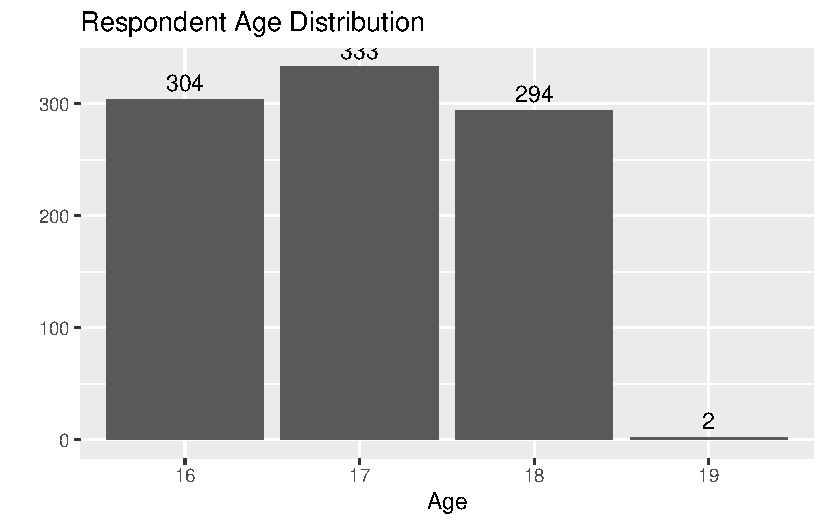
\includegraphics{final_draft_files/figure-pdf/age-1.pdf}

}

\end{figure}

\begin{Shaded}
\begin{Highlighting}[]
\CommentTok{\# save to png file for reports}
\FunctionTok{ggsave}\NormalTok{(}\StringTok{"figures/admissions\_data\_summaries\_age.png"}\NormalTok{)}
\end{Highlighting}
\end{Shaded}

\begin{verbatim}
Saving 5.5 x 3.5 in image
\end{verbatim}

We also asked respondents to self-identify their gender, ethnic group
and religion. Distribution across these categories was as follows:

\begin{Shaded}
\begin{Highlighting}[]
\NormalTok{q16\_labels }\OtherTok{\textless{}{-}} \FunctionTok{c}\NormalTok{(}\StringTok{"Male"}\OtherTok{=}\DecValTok{1}\NormalTok{, }\StringTok{"Female"}\OtherTok{=}\DecValTok{2}\NormalTok{, }\StringTok{"I identify my gender in another way"}\OtherTok{=}\DecValTok{3}\NormalTok{, }\StringTok{"Prefer not to say"}\OtherTok{=}\DecValTok{4}\NormalTok{)}

\FunctionTok{ggplot}\NormalTok{(admissions\_data, }\FunctionTok{aes}\NormalTok{(}\FunctionTok{factor}\NormalTok{(Q16))) }\SpecialCharTok{+} 
  \FunctionTok{geom\_bar}\NormalTok{() }\SpecialCharTok{+}
  \FunctionTok{geom\_text}\NormalTok{(}\AttributeTok{stat =} \StringTok{"count"}\NormalTok{, }\FunctionTok{aes}\NormalTok{(}\AttributeTok{label =} \FunctionTok{after\_stat}\NormalTok{(count)), }\AttributeTok{vjust =} \SpecialCharTok{{-}}\FloatTok{0.5}\NormalTok{) }\SpecialCharTok{+}
  \FunctionTok{labs}\NormalTok{(}\AttributeTok{title =} \StringTok{"Respondent Gender Self{-}Identification Distribution"}\NormalTok{, }\AttributeTok{x =} \StringTok{"Gender"}\NormalTok{, }\AttributeTok{y =} \StringTok{""}\NormalTok{) }\SpecialCharTok{+} \FunctionTok{scale\_x\_discrete}\NormalTok{(}\AttributeTok{labels =} \FunctionTok{labels}\NormalTok{(q16\_labels))}
\end{Highlighting}
\end{Shaded}

\begin{figure}[H]

{\centering 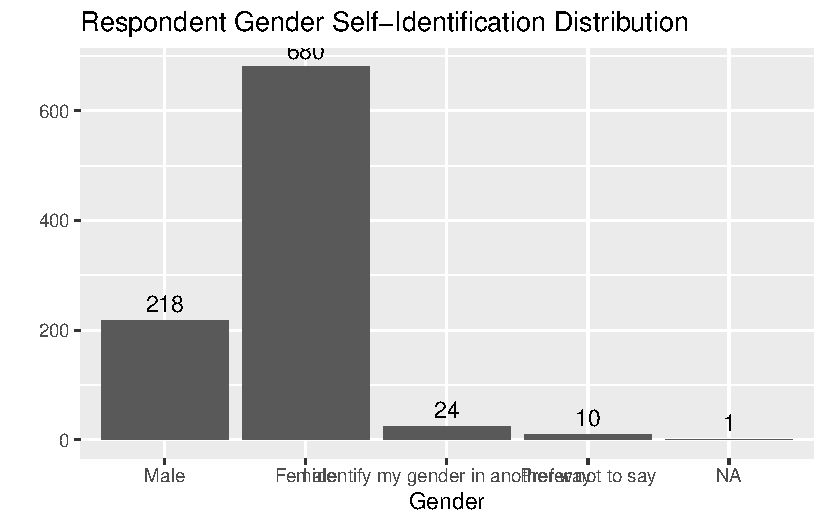
\includegraphics{final_draft_files/figure-pdf/gender-1.pdf}

}

\end{figure}

\begin{Shaded}
\begin{Highlighting}[]
\NormalTok{q17\_labels }\OtherTok{\textless{}{-}} \FunctionTok{c}\NormalTok{(}\StringTok{"Arab"}\OtherTok{=}\DecValTok{1}\NormalTok{, }\StringTok{"Indian"}\OtherTok{=}\DecValTok{2}\NormalTok{, }\StringTok{"Pakistani"}\OtherTok{=}\DecValTok{3}\NormalTok{, }\StringTok{"Bangladeshi"}\OtherTok{=}\DecValTok{4}\NormalTok{, }\StringTok{"Chinese"}\OtherTok{=}\DecValTok{5}\NormalTok{, }\StringTok{"Any other Asian background"}\OtherTok{=}\DecValTok{6}\NormalTok{, }\StringTok{"Black {-} African"}\OtherTok{=}\DecValTok{7}\NormalTok{, }\StringTok{"Black {-} Caribbean"}\OtherTok{=}\DecValTok{8}\NormalTok{, }\StringTok{"Any other Black background"}\OtherTok{=}\DecValTok{9}\NormalTok{, }\StringTok{"Mixed {-} White and Black Caribbean"}\OtherTok{=}\DecValTok{10}\NormalTok{, }\StringTok{"Mixed {-} White and Black African"}\OtherTok{=}\DecValTok{11}\NormalTok{, }\StringTok{"Mixed {-} White and Black Asian"}\OtherTok{=}\DecValTok{12}\NormalTok{, }\StringTok{"Any other Mixed/Multiple Ethnic background"}\OtherTok{=}\DecValTok{13}\NormalTok{, }\StringTok{"White {-} British"}\OtherTok{=}\DecValTok{14}\NormalTok{, }\StringTok{"White {-} Irish"}\OtherTok{=}\DecValTok{15}\NormalTok{, }\StringTok{"Any other White background"}\OtherTok{=}\DecValTok{16}\NormalTok{, }\StringTok{"Prefer not to say"}\OtherTok{=}\DecValTok{17}\NormalTok{, }\StringTok{"Other"}\OtherTok{=}\DecValTok{18}\NormalTok{)}

\FunctionTok{ggplot}\NormalTok{(admissions\_data, }\FunctionTok{aes}\NormalTok{(}\FunctionTok{factor}\NormalTok{(Q17))) }\SpecialCharTok{+}
  \FunctionTok{geom\_bar}\NormalTok{(}\AttributeTok{fill =} \StringTok{"darkgreen"}\NormalTok{, }\AttributeTok{stat =} \StringTok{"count"}\NormalTok{) }\SpecialCharTok{+}
  \FunctionTok{geom\_text}\NormalTok{(}\AttributeTok{stat =} \StringTok{"count"}\NormalTok{, }\FunctionTok{aes}\NormalTok{(}\AttributeTok{label =}\NormalTok{ scales}\SpecialCharTok{::}\FunctionTok{percent}\NormalTok{(}\FunctionTok{after\_stat}\NormalTok{(count }\SpecialCharTok{/} \FunctionTok{sum}\NormalTok{(count)))), }\AttributeTok{vjust =} \SpecialCharTok{{-}}\FloatTok{0.5}\NormalTok{, }\AttributeTok{size=}\FloatTok{2.5}\NormalTok{) }\SpecialCharTok{+}  
  \FunctionTok{labs}\NormalTok{(}\AttributeTok{title =} \StringTok{"Respondent Ethnicity"}\NormalTok{, }\AttributeTok{x =} \StringTok{"Ethnicity"}\NormalTok{, }\AttributeTok{y =} \StringTok{""}\NormalTok{) }\SpecialCharTok{+}
  \FunctionTok{theme}\NormalTok{(}\AttributeTok{axis.text.x =} \FunctionTok{element\_text}\NormalTok{(}\AttributeTok{angle =} \DecValTok{90}\NormalTok{, }\AttributeTok{hjust =} \DecValTok{1}\NormalTok{, }\AttributeTok{vjust =} \FloatTok{0.5}\NormalTok{), }\AttributeTok{text =} \FunctionTok{element\_text}\NormalTok{(}\AttributeTok{size =} \DecValTok{10}\NormalTok{)) }\SpecialCharTok{+} \FunctionTok{scale\_x\_discrete}\NormalTok{(}\AttributeTok{labels =} \FunctionTok{labels}\NormalTok{(q17\_labels))}
\end{Highlighting}
\end{Shaded}

\begin{figure}[H]

{\centering 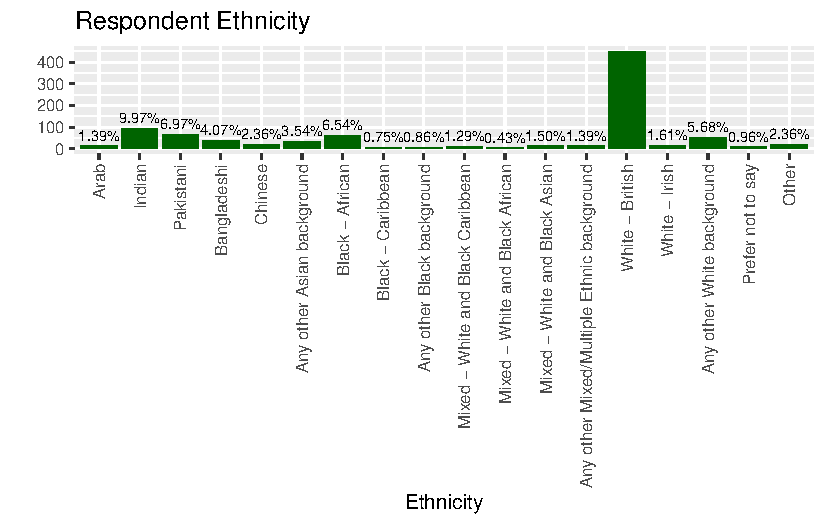
\includegraphics{final_draft_files/figure-pdf/ethnicity-1.pdf}

}

\end{figure}

\begin{Shaded}
\begin{Highlighting}[]
\NormalTok{q18\_labels }\OtherTok{\textless{}{-}} \FunctionTok{c}\NormalTok{(}\StringTok{"Agnostic"}\OtherTok{=}\DecValTok{1}\NormalTok{, }\StringTok{"Atheist"}\OtherTok{=}\DecValTok{2}\NormalTok{, }\StringTok{"Buddhist"}\OtherTok{=}\DecValTok{4}\NormalTok{, }\StringTok{"Christian"}\OtherTok{=}\DecValTok{5}\NormalTok{, }\StringTok{"Confucian"}\OtherTok{=}\DecValTok{6}\NormalTok{, }\StringTok{"Jain"}\OtherTok{=}\DecValTok{7}\NormalTok{, }\StringTok{"Jewish"}\OtherTok{=}\DecValTok{8}\NormalTok{, }\StringTok{"Hindu"}\OtherTok{=}\DecValTok{9}\NormalTok{, }\StringTok{"Muslim"}\OtherTok{=}\DecValTok{11}\NormalTok{, }\StringTok{"Pagan"}\OtherTok{=}\DecValTok{12}\NormalTok{, }\StringTok{"Shinto"}\OtherTok{=}\DecValTok{13}\NormalTok{, }\StringTok{"Sikh"}\OtherTok{=}\DecValTok{14}\NormalTok{, }\StringTok{"Spiritual but not religious"}\OtherTok{=}\DecValTok{15}\NormalTok{, }\StringTok{"Zoroastrian"}\OtherTok{=}\DecValTok{16}\NormalTok{, }\StringTok{"No religion"}\OtherTok{=}\DecValTok{17}\NormalTok{, }\StringTok{"Other"}\OtherTok{=}\DecValTok{18}\NormalTok{)}

\FunctionTok{ggplot}\NormalTok{(admissions\_data, }\FunctionTok{aes}\NormalTok{(}\FunctionTok{factor}\NormalTok{(Q18))) }\SpecialCharTok{+}
  \FunctionTok{geom\_bar}\NormalTok{(}\AttributeTok{fill =} \StringTok{"blue"}\NormalTok{, }\AttributeTok{stat =} \StringTok{"count"}\NormalTok{) }\SpecialCharTok{+}
  \FunctionTok{geom\_text}\NormalTok{(}\AttributeTok{stat =} \StringTok{"count"}\NormalTok{, }\FunctionTok{aes}\NormalTok{(}\AttributeTok{label =}\NormalTok{ scales}\SpecialCharTok{::}\FunctionTok{percent}\NormalTok{(}\FunctionTok{after\_stat}\NormalTok{(count }\SpecialCharTok{/} \FunctionTok{sum}\NormalTok{(count)))), }\AttributeTok{vjust =} \SpecialCharTok{{-}}\FloatTok{0.5}\NormalTok{, }\AttributeTok{size=}\FloatTok{2.5}\NormalTok{) }\SpecialCharTok{+}  
  \FunctionTok{labs}\NormalTok{(}\AttributeTok{title =} \StringTok{"Respondent Religion"}\NormalTok{, }\AttributeTok{x =} \StringTok{"Religion"}\NormalTok{, }\AttributeTok{y =} \StringTok{""}\NormalTok{) }\SpecialCharTok{+}
  \FunctionTok{theme}\NormalTok{(}\AttributeTok{axis.text.x =} \FunctionTok{element\_text}\NormalTok{(}\AttributeTok{angle =} \DecValTok{90}\NormalTok{, }\AttributeTok{hjust =} \DecValTok{1}\NormalTok{, }\AttributeTok{vjust =} \FloatTok{0.5}\NormalTok{), }\AttributeTok{text =} \FunctionTok{element\_text}\NormalTok{(}\AttributeTok{size =} \DecValTok{10}\NormalTok{)) }\SpecialCharTok{+}
  \FunctionTok{scale\_x\_discrete}\NormalTok{(}\AttributeTok{labels =} \FunctionTok{labels}\NormalTok{(q18\_labels))}
\end{Highlighting}
\end{Shaded}

\begin{figure}[H]

{\centering 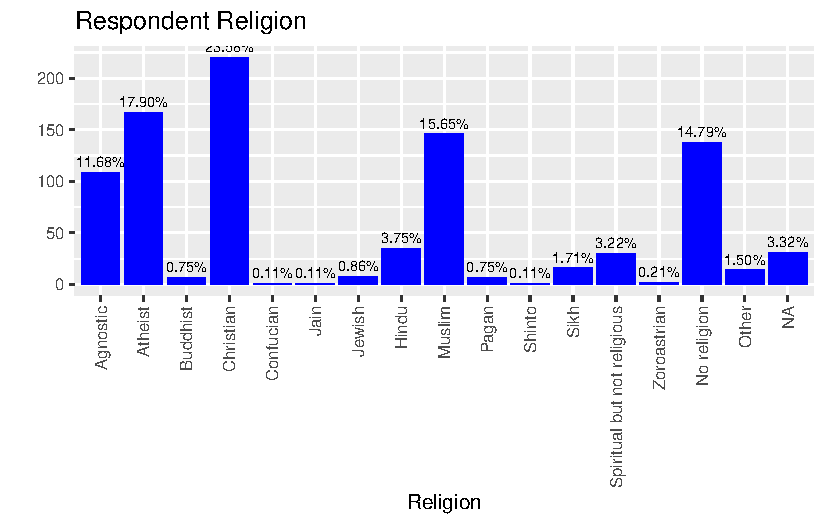
\includegraphics{final_draft_files/figure-pdf/religion-1.pdf}

}

\end{figure}

and

When you click the \textbf{Render} button a document will be generated
that includes both content and the output of embedded code. You can
embed code like this:

\begin{Shaded}
\begin{Highlighting}[]
\DecValTok{1} \SpecialCharTok{+} \DecValTok{1}
\end{Highlighting}
\end{Shaded}

\begin{verbatim}
[1] 2
\end{verbatim}

You can add options to executable code like this

\begin{verbatim}
[1] 4
\end{verbatim}

The \texttt{echo:\ false} option disables the printing of code (only
output is displayed).

\hypertarget{appendix-a-instrument}{%
\section{Appendix A: Instrument}\label{appendix-a-instrument}}



\end{document}
